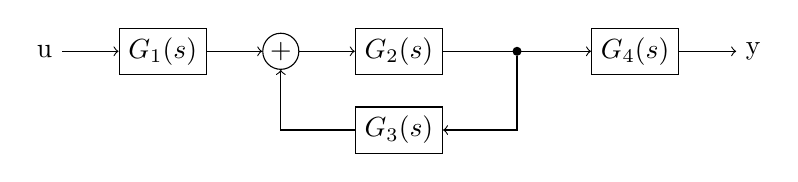
\begin{tikzpicture}
  \node (in) at (0,2) []{u};
  \node (G1) at (1.5,2) [draw]{$G_1(s)$};

  \node (sum) at (3,2) [circle,draw,inner sep=1]{+};

  \node (G2) at (4.5,2) [draw]{$G_2(s)$};
  \node (G3) at (4.5,1) [draw]{$G_3(s)$};

  \node (dot) at (6,2) [draw,circle,inner sep=1,fill]{};
  \node (G4) at (7.5,2) [draw]{$G_4(s)$};
  \node (out) at (9,2) []{y};


  \draw[->] (in) -- (G1);
 
  \draw[->] (G1) --  (sum);
  \draw[->] (sum) --  (G2);

  \draw (G2) -- (dot);
  \draw[->] (dot) |-(G3);
  \draw[->] (G3) -| (sum);

  \draw[->] (dot) |-  (G4);
  \draw[->](G4) -- (out);

\end{tikzpicture}

